\glsreset{DTM}
\glsreset{RF}
\glsreset{MSC}
\glsreset{GTR}
\glsreset{MSA}
\glsreset{ML}
\glsreset{ILS}
\section{Introduction}
In Chapter~\ref{chapter:njmerge}, we proposed an alternative approach to divide-and-conquer that operates by
\begin{enumerate*}[label=(\roman*)]
	\item 
	dividing the species set into pairwise disjoint subsets of a predetermined maximum size, 
	\item 
	estimating a tree on each subset, 
	\item
	computing any auxiliary data required for \glspl{merge} subset trees, and then
	\item
	 using the auxiliary data to merge the subset trees together into a \gls{compatibilitysupertree} (Definition~\ref{def:compatibility-supertree}).
\end{enumerate*}
For the final step, we presented \gls{NJMerge}, a \gls{DTM} method that uses a \gls{dissimilaritymatrix} to build a (possibly refined) compatibility supertree for the subset trees.
Despite its promising theoretical and empirical results, NJMerge has two major issues that limit its utility in practice.
First, NJMerge can fail to return a tree, and second, the worst-case running time of NJMerge is $O(n^4k)$, where the input has $n$ species (leaf labels) divided across $k$ \gls{leaf-label-disjoint} trees.

In this chapter, we address the limitations of NJMerge by presenting new methods, all of which are guaranteed to return a compatibility supertree when given (\gls{fullyresolved}) leaf-label-disjoint trees as input.
The first method, NJMerge-2, is a minor modification to NJMerge; it has the same theoretical properties as NJMerge except that it does not fail.
The second method, \textit{\gls{TreeMerge}}, seeks to address the scalability issue by merging subset trees in two phases: a \textit{\gls{localmergephase}} and a \textit{\gls{globalmergephase}}.
In the local merge phase, a highly accurate but computationally intensive method is used to merge leaf-label-disjoint trees in an embarrassingly parallel fashion. 
In the global merge phase, the trees computed during the local merge phase are then combined via a reduction.
Within the divide-and-conquer framework, TreeMerge runs in $O(n \log{n})$ time or in $O(n^2)$ time if the reduction is serialized. 
This running time analysis assumes that the mergers during the global phase are performed using a linear-time technique.

As we will show, the linear-time merge operation constrains the space of allowed solutions, which in turn places some additional (but achievable) requirements for divide-and-conquer pipelines using TreeMerge to be \gls{statisticallyconsistent} (as compared to those using NJMerge or NJMerge-2).
Nevertheless, the results of our simulation study show that \glspl{speciestree} estimated using TreeMerge can be quite accurate, comparing favorably to those estimated by other DTM-based divide-and-conquer pipelines or traditional species tree estimation methods (\gls{ASTRAL}-III and \gls{CA-ML} using \gls{RAxML}).
Like NJMerge, TreeMerge enables the dominant species tree estimation methods to scale to larger datasets without sacrificing accuracy.
Unlike NJMerge, TreeMerge is guaranteed to return a compatibility supertree, is much faster (in terms of its worst-case running time), and is more easily parallelizable, making it a notable advance for large-scale \gls{phylogeny} estimation.

\section{Approach}
\label{sec:approach}
We now present the NJMerge-2 and TreeMerge algorithms focusing on worst-case running time, correctness, and statistical consistency within divide-and-conquer pipelines.

\subsection{NJMerge-2} 
NJMerge-2 is a simple extension to NJMerge so that it is guaranteed to return a compatibility supertree for the input constraint (subset) trees.
Recall that NJMerge modifies \gls{NJ} by imposing a set of topological constraints on the output tree.
For each siblinghood proposal, NJMerge updates the constraint trees based on the proposed siblinghood and then tests the compatibility of the updated constraint trees; if the test passes, NJMerge accepts the siblinghood proposal.
Because determining the compatibility of a set of  $k$ unrooted trees on overlapping leaf label sets is NP-complete \cite{steel1992complexity}, NJMerge uses a heuristic that can fail for $k > 2$ trees.
Therefore, by running NJMerge on two constraint trees at a time, it will never fail; this observation is the basis of NJMerge-2 (Algorithm~\ref{alg:njmerge2}). 

\begin{theorem}
\label{thm:njmerge2-rt-correct}
Let $\mathcal{T} = \{T_1, T_2, \dots, T_k\}$ be a set of \gls{unrooted} \glspl{phylogenetictree} such that $S(T_i) \cap S(T_j) = \emptyset$ for all $i \ne j$, and let $D$ be an $n \times n$ \gls{dissimilaritymatrix}  on label set $S = \cup_{i=1}^k S(T_i)$.
Then, NJMerge-2 applied to input $(\mathcal{T}, D)$ returns a (possibly refined) compatibility supertree for $\mathcal{T}$ in $O(n^4k)$ time; the parallel version of NJMerge-2 runs in $O(n^4)$ time.
Furthermore, if $D$ is a \gls{nearlyadditive} matrix for a fully resolved tree $T^*$ on label set $S$ (Definition~\ref{def:nearly-additive}) and if $T^*$ is \gls{compatible} with $T_i$ for all $i \in \{1, \dots, k\}$ (Definition~\ref{def:compatibility}), then NJMerge-2 returns $T^*$.
\end{theorem}

\begin{proof}
\emph{Returns a compatibility supertree:} It is easy to see that the constraint trees remain leaf-label-disjoint and thus compatible at each iteration, and because the heuristics used by NJMerge correctly determine compatibility for two trees, NJMerge applied to the input $\big( \{ t, t' \}, D|_{S(t) \cup S(t')} \big)$ is guaranteed to return a (possibly refined) compatibility supertree (Theorem~\ref{thm:njmerge}).
By induction on the number of constraint trees, NJMerge-2 returns a (possibly refined) compatibility supertree for $\mathcal{T}$.

\emph{Correctness:} If, in addition, the trees in $\mathcal{T}$ are compatible with $T^*$ and the dissimilarity matrix $D$ is nearly additive for $T^*$, then for any pair of trees $t, t' \in \mathcal{T}$, NJMerge applied to the input $\big( \{ t, t' \}, D|_{S(t) \cup S(t')} \big)$ returns $T^*|_{S(t) \cup S(t')}$ (Theorem~\ref{thm:njmerge-correct}).
Therefore, the set $\mathcal{T}$ remains compatible with $T^*$ during the iterative process.
By induction on the number of constraint trees, NJMerge-2 returns $T^*$.

\emph{Running time:} For the running time analysis, we make the simplifying assumption that each of the $k$ trees in $\mathcal{T}$ has exactly $n/k$ leaves.
At iteration $w$, for any two trees $t, t' \in \mathcal{T}$, $ |S(t) \cup S(t') | \le (w + 1)n/k$, so the worst-case running time of NJMerge given any pair of trees is $O(w^4 n^4 / k^4)$ (Theorem~\ref{thm:njmerge}).
A total of $k-1$ iterations are required, so the running time of NJMerge-2 scales with $(n^4/k^4) \sum_{w=2}^k w^4$. 
Because $\sum_{w=2}^k w^4$ is $O(k^5)$, the worst-case running time of NJMerge-2 is $O(n^4k)$. Although Algorithm~\ref{alg:njmerge2} runs NJMerge-2 on pairs of trees in serial, we could consider a parallel version of NJMerge-2. 
Assuming that $k$ is a power of two for simplicity, at iteration $w$, we run NJMerge on each of the $k/(2^w)$ pairs of trees in parallel, where for any pair of trees  $t, t' \in \mathcal{T}$, $ |S(t) \cup S(t') | = 2^{w}n/k$.
A total of $p = \log_2{(k)} - 1$ iterations are required, so the parallel running time of NJMerge scales with $(n^4/k^4) \sum_{w=2}^p 2^{4w}$ and thus is $O(n^4)$.
This is expected as the running time of NJMerge-2 is dominated by the time to run NJMerge in the final iteration.
\end{proof}

\vspace{12pt}

\begin{algorithm}[!h]
\footnotesize
\setstretch{1.15}
\caption{{\bf NJMerge-2.}}
\label{alg:njmerge2}
\DontPrintSemicolon
\SetAlgoNoLine
\SetAlgoNoEnd
\SetKwInOut{Input}{Input}
\SetKwInOut{Output}{Output} 
\SetKwFunction{NJMerge}{NJMerge}
\SetKwFunction{NJMergeTwoSerial}{NJMergeTwoSerial}
\SetKwFunction{SelectPair}{SelectPair}
\SetKwFunction{CopyMatrixRestricted}{CopyMatrixRestricted}
\SetKwFunction{DeleteMatrix}{DeleteMatrix}
\SetKwProg{Pn}{Function}{:}{}
\vspace{.1in}
 \Input{Set $\mathcal{T} = \{T_i \}_{i=1}^k$ of  unrooted phylogenetic tree such that $S(T_i) \cap S(T_j) = \emptyset$ for all $i \ne j$ and an $n \times n$ dissimilarity matrix $D$ on label set $S_{i=1}^k \bigcup S_i$}
\Output{A (possibly refined) compatibility supertree for $\mathcal{T}$ that is fully resolved}
\vspace{-4pt}

\hrulefill

\Pn{\NJMergeTwoSerial{$\mathcal{T}$, $D$, $S$}}{
	\While{$|\mathcal{T}| > 1$}{
		\vspace{10pt}
		$t, t' \leftarrow$ An arbitrary pair of trees in $\mathcal{T}$\;
		$R \leftarrow [S(t) \cup S(t')]$\;
		$D|_R \leftarrow$ \CopyMatrixRestricted{$D$, $R$} \;
		%\vspace{10pt}
		$T \leftarrow$ \NJMerge{$\{ t, t' \}$, $D|_R$, $R$}\;
		%\vspace{10pt}
		\DeleteMatrix{$D|_R$}\;
		%\vspace{10pt}
		$\mathcal{T} \leftarrow \big( \mathcal{T} \setminus \{ t, t' \} \big) \cup \{ T \}$\;
		\vspace{10pt}
	}
	\Return{$T$}\;
 }
 \vspace{3pt}
\end{algorithm}

We do not specify an order for merging pairs of constraint trees in Algorithm~\ref{alg:njmerge2}.
While the order does not impact the theoretical guarantees of NJMerge-2, it likely impacts performance (accuracy) in practice. 
Consider a collection of constraint trees that are \gls{edgeseparable} for a \gls{caterpillartree} $T$ with a very large \textit{\gls{evolutionarydiameter}} (the longest evolutionary distance between any pair of leaves in a phylogenetic tree).
If, in the first iteration, we merge two constraint trees on opposite sides of the caterpillar tree, the output tree may contain incorrect \glspl{bipartition} due to \gls{longbranchattraction}; these incorrect bipartitions will be propagated through subsequent iterations.
Hence, it may be beneficial to perform mergers in an order that respects locality by selecting pairs of trees $t, t' \in \mathcal{T}$ based on the evolutionary distance between set $S(t)$ and set $S(t')$ in $D$. 
Exploiting locality can also be useful for improving computationally efficiency, as we will show.

\subsection{TreeMerge}
\label{sec:treemerge}
\glsreset{TreeMerge}
We now introduce TreeMerge, the first DTM method that combines an embarrassingly parallel local merge phase with a global merge phase.
As shown in Algorithm~\ref{alg:treemerge}, these two phases are enabled through the use of a \textit{\gls{mergeguidetree}} given as part of the input.
The generic TreeMerge algorithm also requires auxiliary data in order to build compatibility supertrees during both the local and the global merge phases.
The exact details of the algorithm can be implemented in a variety of ways; we present two examples: TreeMerge-fast (which was previously mentioned) and TreeMerge-slow.

\begin{itemize}
	\item \textbf{\gls{TreeMergeinput}}: 
	\begin{itemize}
		\item Set $\mathcal{T} = \{T_1, T_2, \dots, T_k\}$ of \gls{unrooted}, \gls{fullyresolved} \glspl{phylogenetictree} such that $S(T_i) \cap S(T_j) = \emptyset$ for all $i \ne j$
		\item Set $\mathcal{A}$ of auxiliary data, including
		\begin{itemize}
			\item \Gls{mergeguidetree} $\mathcal{G}$ with nodes bijectively labeled by elements of the set $\{1, 2, \dots, k\}$ such  that node $i$ corresponds to tree $T_i \in \mathcal{T}$
			\item Data that can be used to merge trees, for example
			\begin{itemize}
				\item {\em TreeMerge-fast:} Set $\mathcal{D} = \{ D^{i,j} : (i,j) \in E(\mathcal{G}) \}$ of \glspl{dissimilaritymatrix}
				\item {\em TreeMerge-slow:} Dissimilarity matrix $D$ on label set $S = \bigcup_{i=1}^k S(T_i)$
			\end{itemize}
		\end{itemize}
	\end{itemize}
	\item \textbf{\gls{TreeMergeoutput}}: \Gls{compatibilitysupertree} for $\mathcal{T}$ %that is fully resolved
\end{itemize}

\begin{algorithm}[!h]
\footnotesize
\setstretch{1.15}
\caption{{\bf Generic TreeMerge Algorithm.}}
\label{alg:treemerge}
\DontPrintSemicolon
\SetAlgoNoLine
\SetAlgoNoEnd
\SetKwInOut{Input}{Input}
\SetKwInOut{Output}{Output} 
\SetKwFunction{NJMerge}{NJMerge}
\SetKwFunction{GenericTreeMerge}{GenericTreeMerge}
\SetKwFunction{PreOrderEdgeTraversal}{PreOrderEdgeTraversal}
\SetKwFunction{UpdateTree}{UpdateTree}
\SetKwFunction{RootTreeAtEdge}{RootTreeAtEdge}
\SetKwProg{Pn}{Function}{:}{}
\vspace{.1in}
 \Input{
Set $\mathcal{T} = \{T_1, T_2, \dots, T_k\}$ of unrooted, fully resolved phylogenetic trees with constraint tree $T_i$ on label set $S_i$ such that $S_i \cap S_j = \emptyset$ for all $i \ne j$, a set $\mathcal{A}$ of auxiliary data, which includes a tree $\mathcal{G}$, called the merge guide tree, with nodes bijectively labeled by elements of the set $\{1, 2, \dots, k \}$ so that node $i$ corresponds to tree $T_i \in \mathcal{T}$.
 }
\Output{Compatibilitysupertree for $\mathcal{T}$}
\vspace{-4pt}

\hrulefill

\Pn{\GenericTreeMerge{$\mathcal{T}$, $\mathcal{A}$}}{
	\vspace{10pt}
	{\bf Local merge phase:} For each edge $(i, j) \in E(\mathcal{G})$, build a compatibility supertree $T_{i,j}$ for $\{T_i, T_j\}$ using some auxiliary data in $\mathcal{A}$\;
	\vspace{10pt}
	{\bf Global merge phase:} \;
	$(x,y) \leftarrow $ An arbitrary edge in $E(\mathcal{G})$\;
	$T \leftarrow T_{x,y}$\;
	$\mathcal{G} \leftarrow$ $\mathcal{G}$ rooted at edge $(x,y)$\;
	\For{$(i, j) \in$ \PreOrderEdgeTraversal{$\mathcal{G}$}}{
		%\vspace{10pt}
		$T \leftarrow$ Compatibility supertree for $\{T, T_{i,j}\}$ built using their \gls{backbonetree} $T|_{S(T) \cap S(T_{i,j})}$ and possibly some auxiliary data in $\mathcal{A}$\;
	}
	\vspace{10pt}
	\Return{$T$}\;
 }
\vspace{3pt}
\end{algorithm}

\vspace{6pt}

We now describe the local and global phases for TreeMerge-slow and TreeMerge-fast.

\paragraph{Local merge phase:} 
During the local merge phase, mergers are performed on pairs of trees that are local, meaning that they are connected by edges in the merge guide tree $\mathcal{G}$.
For every edge $(i, j) \in E(\mathcal{G})$, both TreeMerge-slow and TreeMerge-fast build a compatibility supertree $T_{i,j}$  by running NJMerge on the input $(\{T_i,T_j\}, D^{i,j})$.
Afterward, TreeMerge-fast uses $D^{i,j}$ to fit branch lengths to $T_{i,j}$ via the least squares approach proposed by Bryant and Waddell \cite{bryant1998rapid}.
Note that TreeMerge-fast takes $D^{i,j}$ as input, whereas TreeMerge-slow creates $D^{i,j}$ by restricting $D$ to label set $S(T_i) \cup S(T_j)$.

\paragraph{Global merge phase:} 
During the global merge phase, mergers are performed following a pre-order edge traversal of the merge guide tree $\mathcal{G}$, combining the trees computed during the local merge phase into a single tree on label set $S$ (note that this can also be implemented as a reduction; see Figure \ref{fig:reduction} for an example).
The merge technique is related to the Strict Consensus Merger \cite{warnow2001absolute, swenson2012superfine}.

We describe this merge technique in the context of merging two trees $T_{i,j}$ and $T_{j,k}$ that are compatibility supertrees for $\{T_i, T_j\} \subset \mathcal{T}$ and $\{T_j, T_k\} \subset \mathcal{T}$, respectively.
The input trees in $\mathcal{T}$ are fully resolved, so $T_{i,j}$ and $T_{j,k}$ 
%are fully resolved and thus 
induce a common tree \gls{topology} $T_j$ when restricted to their shared label set; we refer to $T_j$ as the \textit{\gls{backbonetree}}.
Each edge $e$ in $E(T_j)$ maps to a path $p_{i,j}(e)$ in $T_{i,j}$ and a path $p_{j,k}(e)$ in $T_{j,k}$.
When $p_{i,j}(e)$ or $p_{j,k}(e)$ have length greater than one, the internal nodes on those paths define subtrees that need to be inserted onto edge $e$ in the backbone tree $T_j$.
Let $V_{i,j}(e)$ denote the set of subtrees in $T_{i,j}$ that need to be attached to edge $e$, and similarly, let $V_{j,k}(e)$ denote the set of subtrees in $T_{j,k}$ that need to be attached to edge $e$.
It is easy to see that adding subtrees in the set $V_{i,j}(e) \cup V_{j,k}(e)$ to edge $e$ in an arbitrary order and then repeating this process for all edges in $E(T_j)$, produces a (possibly refined) compatibility supertree for $\{T_{i,j}, T_{j,k} \}$ and thus for $\{ T_i, T_j, T_k \}$.
If $T_{i,j}$ and $T_{j,k}$ never contribute subtrees to the same edge, $T_{i,j,k}$ is the unique compatibility supertree for $\{ T_i, T_j, T_k \}$; otherwise, $T_{i,j,k}$ is a refined compatibility supertree.

When $T_{i,j}$ and $T_{j,k}$ both contribute subtrees to the same edge (referred to as a \textit{\gls{collision}}), there are multiple ways to merge the two trees while maintaining compatibility (Figure \ref{fig:slow-vs-fast}).
Picking the best resolution cannot be done using tree topologies of $T_{i,j}$ and $T_{j,k}$ alone.
TreeMerge-fast and TreeMerge-slow differ with respect to how they resolve collisions.

\paragraph{TreeMerge-fast:}
TreeMerge-fast resolves edge collisions by using the branch lengths fitted to $T_{i,j}$ and $T_{j,k}$ during the local merge phase.
Suppose that $T_{i,j}$ and $T_{j,k}$ each contribute one or more subtrees to an edge $e$ in their shared backbone tree $T_j$.
Then, edge $e$ has two different lengths: the length given by path $p_{i,j}(e)$ in $T_{i,j}$ and the length given by path $p_{j,k}(e)$ in $T_{j,k}$.
TreeMerge-fast rescales these paths so that they have same length, producing an order for subtrees in $V_{i,j}(e) \cup V_{j,k}(e)$ to be added to edge $e$.
This approach does not allow subtrees contributed by $T_{i,j}$ and $T_{j,k}$ to \gls{blend} together (Figure \ref{fig:slow-vs-fast}), limiting the potential solutions that can be returned by TreeMerge-fast.
It is not possible for TreeMerge-fast to recover the correct tree for some subset decomposition and merge guide tree pairs (Figure~\ref{fig:collisions}).

\paragraph{TreeMerge-slow:}
TreeMerge-slow resolves edge collisions between two trees $T_{i,j}$ and $T_{j,k}$ using the shared backbone tree $T_j$ as follows.
Let $e =(X',Y') \in E(T_j)$ be an edge involved in a collision, and select two labels $X, Y \in S(T_j)$ corresponding to leaves on opposite sides of $e$.
We define a constraint tree $t$ by restricting $T_{i,j}$ to leaf label set $\{ X, Y \} \cup \{ S(v) : v \in V_{i,j}(e) \}$, and we define another constraint tree $t'$ by restricting $T_{j,k}$ to leaf label set $\{ X, Y \} \cup \{ S(v) : v \in V_{j,k}(e) \}$.
Because $t$ and $t'$ have only leaves $X$ and $Y$ in common, they are compatible; therefore, a compatibility supertree for $\{t, t'\}$ can be computed in polynomial time by running NJMerge on the input $\big(\{ t, t' \}, D_{S(t) \cup S(t')})$ (Theorem~\ref{thm:njmerge}).
The compatibility supertree for $\{ t,t' \}$ can be inserted into $T_j$ by attaching leaf $X$ at node $X'$ and leaf $Y$ at node $Y'$.
This technique allows $t$ and $t'$ to blend (Figure~\ref{fig:slow-vs-fast}).

\begin{landscape}
\begin{figure}
\centering
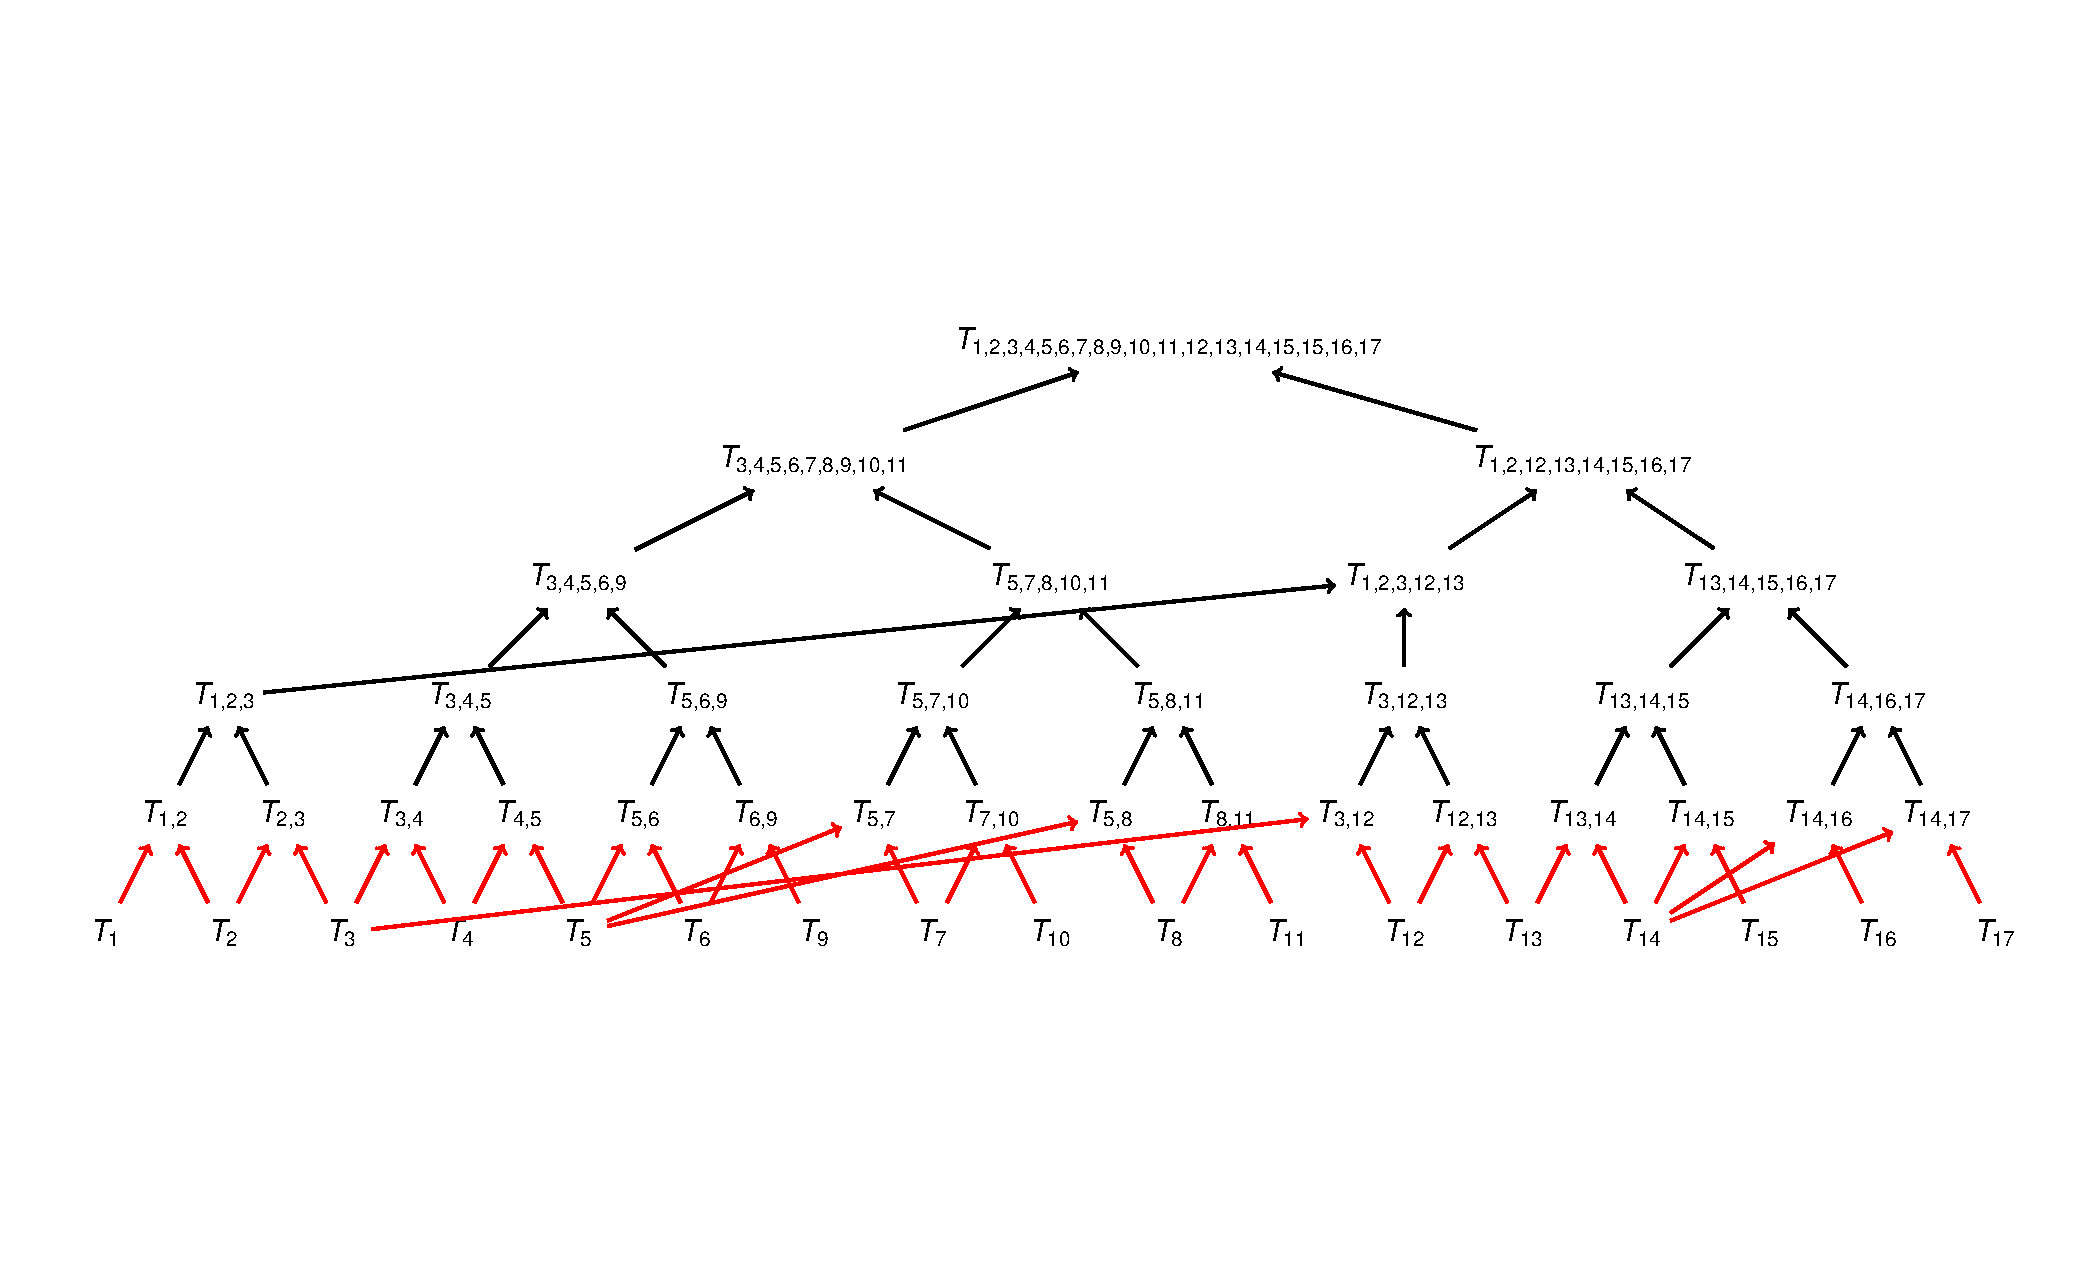
\includegraphics[scale=0.65]{figures/treemerge-fig1.pdf}
\captionsetup{singlelinecheck=off}
\caption[]{{\bf Parallel Reduction for the Generic TreeMerge.} 
It is well known that a reduction can be performed on a tree. This reduction is for subset trees $\mathcal{T} = \{T_1, T_2, \dots, T_{17} \}$ and merge guide tree $\mathcal{G}$ given by edge set: $\{(1,2), (2,3), (3,4), (4,5), (5,6), (6,9), (5,7), (7,10), (5,8), (8,11), (3,12), (12,13), (13, 14), (14, 15), (14, 16), (14, 17)\}$.
Red arrows indicate that two trees (e.g., $T_{14}$ and $T_{17}$) are given as input to a DTM method (e.g., using NJMerge). Black arrows indicate that two trees (e.g., $T_{14,17}$ and $T_{14,16}$) are merged via their shared backbone tree (e.g., using branch lengths as in TreeMerge-fast). The local merge phase is one step (red arrows), and the global merge phase takes $\log_2{(16)} = 4$ steps (black arrows). Mergers at each of these steps can be performed in an embarrassingly parallel fashion.}
\label{fig:reduction}
\end{figure}
\fillandplacepagenumber
\end{landscape}

\glsreset{blend}
\begin{figure}[!h]
\centering
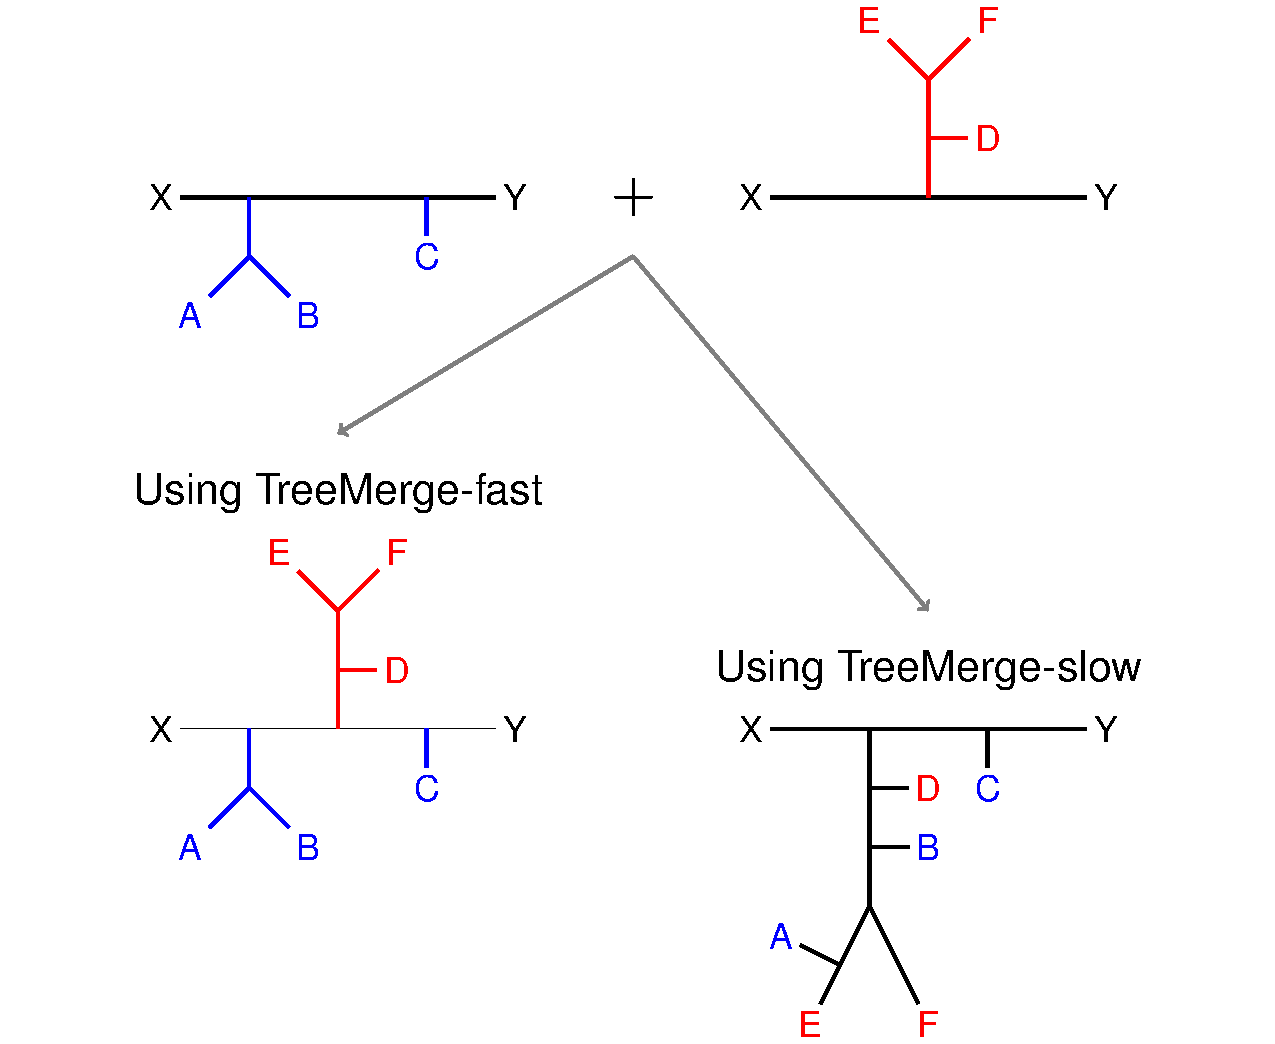
\includegraphics[width=0.9\textwidth]{figures/treemerge-fig2.pdf}
\caption{
{\bf TreeMerge-slow vs. TreeMerge-fast. }
TreeMerge-slow and TreeMerge-fast differ with respect to how they resolve edge collisions.
Consider the case where two compatible trees $T_{i,j}$ and $T_{j,k}$ are involved in a collision on edge $e = (X', Y')$ in the backbone tree $T_j$, using the notation from Section \ref{sec:treemerge}.
Select two leaves $X$ and $Y$ on opposite sides of the edge $e$ in $T_j$.
We define a constraint tree $t$ (upper left corner) by restricting $T_{i,j}$ to leaf label set $\{ x, y \} \cup \{ S(v) : v \in V_{i,j}(e) \}$, 
so the subtrees in $V_{i,j}(e)$ are given by the \gls{newick} strings: $(A,B)$ and $(C)$.
We define another constraint tree $t'$ (upper right corner) by restricting $T_{j,k}$ to leaf label set $\{ x, y \} \cup \{ S(v) : v \in V_{j,k}(e) \}$, so the one subtree in $V_{i,k}(e)$ is given by the Newick string: $(D,(E,F))$.
The goal is to produce a compatibility supertree $t^*$ for $\{ t, t' \}$ and then insert $t$ into the backbone tree $T_j$ by attaching leaf $X$ at \gls{internalnode} $X'$ and attaching leaf $Y$ at internal node $Y'$.
TreeMerge-fast builds $t^*$ by rescaling branch lengths (if necessary) so that the paths from $X$ to $Y$ in $t$ and $t'$ have the same length (as shown here); $t$ is then defined by superimposing these paths.
When resolving collisions, TreeMerge-fast does not allow \textit{\glspl{blend}}, because the subtrees in the set $V_{i,j}(e) \cup V_{j,k}(e) \cup \{X, Y\}$ must be edge separable for $t^*$.
In contrast, TreeMerge-slow builds $t^*$ by running NJMerge on the input $\big(\{t, t'\}, D|_{S(t) \cup S(t')} \big)$; this enables blending.}
\label{fig:slow-vs-fast}
\end{figure}

\begin{figure}[!h]
\centering
%\includegraphics[width=1.0\textwidth]{figures/treemerge-fig3.pdf}
	\begin{subfigure}[t]{0.45\textwidth}
	\centering
		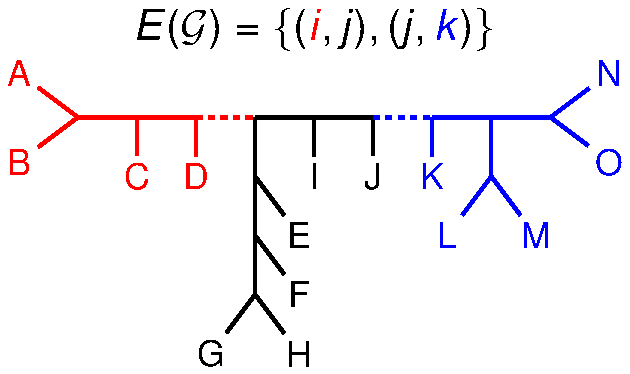
\includegraphics[width=\textwidth]{figures/treemerge-fig3a.pdf}
		~
		\caption{(a) No collisions $\{ T_{i,j}, T_{j,k} \}$} 
	\end{subfigure}
	~~~~~~~~~~
	\begin{subfigure}[t]{0.45\textwidth}
	\centering
		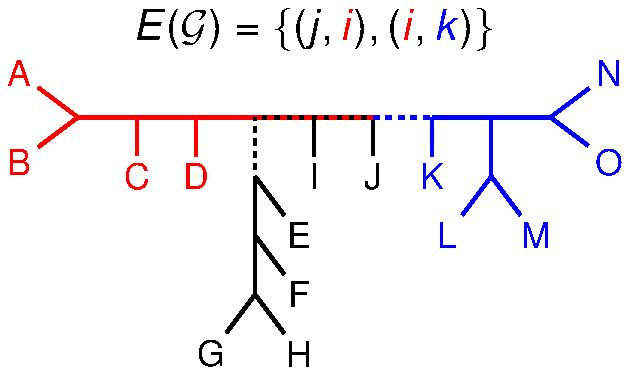
\includegraphics[width=\textwidth]{figures/treemerge-fig3b.pdf}
		~
		\caption{(b) Collisions $\{ T_{j,i}, T_{i,k} \}$} 
	\end{subfigure}

	\vspace{24pt}

	\begin{subfigure}[t]{0.45\textwidth}
	\centering
		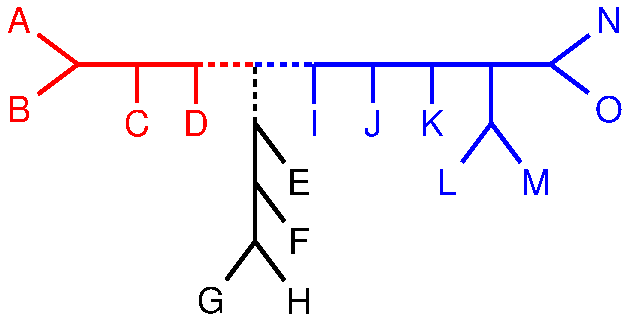
\includegraphics[width=\textwidth]{figures/treemerge-fig3c.pdf}
		~
		\caption{(c) Collision for all $\mathcal{G}$} 
	\end{subfigure}
	~~~~~~~~~~
	\begin{subfigure}[t]{0.45\textwidth}
	\centering
		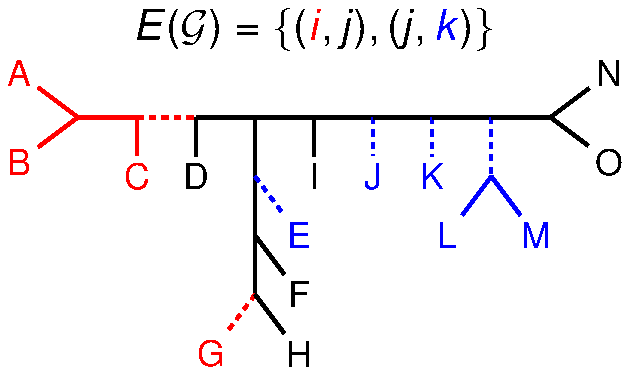
\includegraphics[width=\textwidth]{figures/treemerge-fig3d.pdf}
		~
		\caption{(d) No collisions $\{ T_{i,j}, T_{j,k} \}$} 
	\end{subfigure}
\caption{
{\bf Impact of collisions on the correctness of TreeMerge-fast. }
For each subfigure, the true tree $T$ is shown. 
Colors indicate how the leaves of $T$ have been decomposed into subsets: subset $i$, $j$, and $k$ are shown in red, black, and blue, respectively.
Suppose that subset trees $T_i$, $T_j$, or $T_k$ are correct and thus can be created by restricting $T$ to the red, black, or blue leaves, respectively.
The merge guide tree $\mathcal{G}$ indicates how the TreeMerge algorithm proceeds.
For example, in subfigure (a), $\mathcal{G}$ indicates that $\{T_i, T_j\}$ and $\{T_j, T_k\}$ are merged during the local phase. 
Again, suppose that the resulting trees are correct; therefore, $T_{i,j}$  can be created by restricting $T$ to the red and black leaves, and $T_{j,k}$ can be created by restricting $T$ to the black and blue leaves.
During the global phase, TreeMerge-fast merges $T_{i,j}$ and $T_{j,k}$ via the backbone tree $T_j$. 
Subfigure (a) shows no collisions, so TreeMerge-fast returns the correct tree.
Subfigure (b) shows a collision on the edge with bipartition $A,B,C|D$ in $T_j$, so TreeMerge-fast returns the incorrect tree; for example, TreeMerge-fast could return the tree given by Newick string: ${(\color{red} (A,B),C)},\;(((((G,H),F),E),(I,J)),{\color{blue}(K,((L,M),(O,N)))}),\;{\color{red} D})$.
Note that subfigure (b) shows the same subset decomposition as subfigure (a), but $\mathcal{G}$ is different.
Subfigure (c) shows a collision occurring regardless of $\mathcal{G}$, and TreeMerge returns the incorrect tree for this decomposition regardless of the $\mathcal{G}$; for example, TreeMerge-fast run on $\{ T_{i,j}, T_{i,k} \}$ could return ${(\color{red} ((A,B),C)},\; (((G,H),F),E),\; {\color{blue} (I,(J,(K,((L,M),(O,N)))))}, \; {\color{red} D})$.
Subfigure (d) shows no collisions, so TreeMerge-fast returns the correct tree. Unlike in the other subfigures, the subset trees $\{ T_i, T_j, T_j\}$ are not edge separable for $T$.
 }
\label{fig:collisions}
\end{figure}

\clearpage

We now provide some theoretical guarantees for TreeMerge-fast and TreeMerge-slow.

\begin{theorem}
\label{thm:treemerge-rt}
Suppose that the input $(\mathcal{T}, \mathcal{A})$ has $n$ leaf labels divided across $k$ leaf-label-disjoint trees in $\mathcal{T}$.
Then, TreeMerge-fast applied to $(\mathcal{T}, \mathcal{A})$ returns a compatibility supertree for $\mathcal{T}$ in 
 $O(nk + n^2/k + n^4/k^3)$ time if using the serial version and $O(n \log_2{k} + n^2/k^2 + n^4/k^4)$ time if using the parallel version.
TreeMerge-fast requires $O(n^2 / k)$ storage.

In contrast, TreeMerge-slow applied to $(\mathcal{T}, \mathcal{A})$ returns a compatibility supertree for $\mathcal{T}$ in $O(n^4k)$ time if using the serial version and $O(n^4)$ time if using the parallel version.
TreeMerge-slow requires $O(n^2)$ storage.
\end{theorem}

\begin{proof}
The proof that both TreeMerge-slow and TreeMerge-fast return a compatibility supertree follows from the technique for building compatibility supertrees (in the local merge phase) returning a compatibility supertree when given two leaf-disjoint trees as input and from the techniques for resolving collisions (in the global merge phase) returning a compatibility supertree when given two trees that \gls{agree} on their shared leaf label set.

For the running time analysis, we make the simplifying assumptions that each tree in $\mathcal{T}$ has exactly $n/k$ leaves and that $k-1$ is a power of two.

\emph{Local merge phase:} 
In the local merge phase, both TreeMerge-slow and TreeMerge-fast run NJMerge on input $(\{T_i, T_j\}, D^{i,j})$ for each of the $k-1$ edges in the merge guide tree $\mathcal{G}$.
All input constraint trees have $n/k$ leaves, so the local merge phase uses $O(n^2/k)$ storage.
The running time of the local merge phase is $O(n^4/k^3)$ if mergers are performed in serial and $O(n^4/k^4)$ if mergers are performed in parallel.

\emph{Extended local merge phase for TreeMerge-fast:}
TreeMerge-fast extends the local merge phase by computing branch lengths for each of the $k-1$ trees using the quadratic time and space algorithm from \cite{bryant1998rapid}. 
The running time of the extended local merge phase is then $O(n^2/k)$ if performed in serial and $O(n^2/k^2)$ if performed in parallel.

TreeMerge-fast and TreeMerge-slow implement the global merge phase differently; we discuss these methods separately using the notation from Algorithm~\ref{alg:treemerge}.

\emph{Global merge phase for TreeMerge-fast:}
At iteration $w$, TreeMerge-fast merges trees $T_{i,j}$ and $T$ using their shared backbone tree $t_B$ and branch lengths.
This is just a special case of the algorithm proposed by Bansal \cite{bansal2018linear} for Optimal Tree Completion under the \gls{RF} Distance.
This algorithm scales linearly with the number of leaf labels in the output tree, so $|S(T_{i,j}) \cup S(T)| = (w+2)n/k$.
A total of $k-2$ iterations are required, so the running time scales with $(n/k) \sum_{w=3}^k w$.
Because $\sum_{w=3}^p w$ is $O(p^2)$, the worst-case running time of TreeMerge-fast is $O(kn)$.
It is possible to perform this global merge phase in parallel via a reduction on the merge guide tree $\mathcal{G}$.
We merge trees using branch lengths in $\log_2{(k-1)}$ iterations and each iteration is $O(n)$; therefore, in the parallelized global merge
\clearpage
\noindent phase, TreeMerge-fast uses $O(n \log_2{k})$ time.

\emph{Global merge phase for TreeMerge-slow:}
At iteration $w$, TreeMerge-slow merges trees $T_{i,j}$ and $T$ using their shared backbone tree $t_B$, where $|S(T_{i,j})| = 2n/k$, $|S(T)| = (w + 1)n/k$, and $|S(t_B)| = n/k$.
There are $(w+1)n/k$ possible leaves that could be contributed to the $n/k - 3$ edges in $t_B$.
In the worst case analysis, $(w+1) n / k$ leaves are contributed to a single edge in $t_B$, so NJMerge uses $O(w^4 n^4 / k^4)$ time and $O(w^2 n^2 / k^2)$ storage.
A total of $k-2$ iterations are required, so the running time scales with $(n^4/k^4) \sum_{w=3}^k w^4$.
Because $\sum_{w=3}^p w^4$ is $O(p^5)$, the worst-case running time of TreeMerge-slow is $O(kn^4)$.
In the serialized global merge phase, TreeMerge-slow uses $O(n^4k)$ time and uses $O(n^2)$ storage.
Notably, the worst-case analysis is effectively the same as the analysis for NJMerge-2 (essentially just specifying the order of the mergers).
It is possible to perform the global merge phase in parallel via a reduction on the merge guide tree $\mathcal{G}$; the worst-case analysis is effectively the parallel version of NJMerge-2, so TreeMerge-slow requires $O(n^4)$ time.

Overall, TreeMerge-slow uses $O(n^2)$ storage and TreeMerge-fast uses $O(n^2/k)$ storage.
For the serialized versions, TreeMerge-slow runs in $O(n^4k)$ time and TreeMerge-fast runs in $O(nk + n^2/k + n^4/k^3)$ time.
For the parallelized versions, TreeMerge-slow runs in $O(n^4)$ time and TreeMerge-fast runs in $O(n \log_2{k} + n^2/k^2 + n^4/k^4)$ time.
\end{proof}

Note that while the worst-case running time of TreeMerge-slow is the same as the worst-case running time of NJMerge-2, these two methods can have very different running times in practice, for example when there are very few collisions. 
In fact, when there are zero collisions, TreeMerge-slow and TreeMerge-fast have the same running time.
That being said, it is possible for large collisions to occur; for example, if TreeMerge-slow was run on the case presented in Figure~\ref{fig:collisions}b, it would run NJMerge on two red leaves ($D$ and either $A$, $B$, or $C$), all black leaves, and all blue leaves, so basically the entire tree!

\begin{theorem}
\label{thm:treemerge-slow-correct}
If a phylogenetic tree $T^*$ is compatible with every tree in $\mathcal{T}$, and $D$ is nearly additive for $T^*$.
Then, TreeMerge-slow returns $T^*$.
\end{theorem}

\begin{proof}
Let $T_x$ and $T_y$ be two trees in $\mathcal{T}$.
NJMerge applied to $\big(\{T_x, T_y\}, D|_{S(T_x) \cup S(T_y)}\big)$ returns $T^*|_{S(T_x) \cup S(T_y)}$ by Theorem~\ref{thm:njmerge-correct}.
As TreeMerge-slow performs all its mergers using NJMerge, the result follows by induction on the number of mergers.
\end{proof}

\begin{theorem}
\label{thm:treemerge-fast-correct}
If a phylogenetic tree $T^*$ is compatible with every tree in $\mathcal{T}$, and $D$ is nearly additive for $T^*$. 
Then, TreeMerge-fast is guaranteed to return $T^*$ provided that there are no collisions during the global merge phase.
\end{theorem}

\begin{proof}
If there are no collisions during the global merge phase, TreeMerge-fast performs all of its mergers with NJMerge; the result follows by induction on the number of mergers.
\end{proof}

\subsection{Divide-and-conquer Pipelines for Phylogeny Estimation and Statistical Consistency}
We now provide some theoretical guarantees for divide-and-conquer pipelines that use either NJMerge-2, TreeMerge-slow, or TreeMerge-fast to combine subset trees; see Algorithm~\ref{alg:njmerge-divide-and-conquer}.

\begin{corollary}
When run within the divide-and-conquer framework proposed in Algorithm~\ref{alg:njmerge-divide-and-conquer}, TreeMerge-fast runs in $O(n^2)$ time if using the serial version and $O(n \log_2{n})$ time if using the parallel version.
In contrast, the parallel versions of NJMerge-2 and TreeMerge-slow run in $O(n^4)$ time, and the serial versions of NJMerge, NJMerge-2, and TreeMerge-slow run in $O(n^5)$ time.
\end{corollary}

\begin{proof}
In the divide-and-conquer framework, the input dataset of $n$ species is divided into $k$ pairwise disjoint subsets of bounded size, so $c = n/k$ and therefore $k = n/c = O(n)$.
Then, the result follows from updating the equations for worst-case running time given in Table~\ref{tab:info}.
\end{proof}

\begin{corollary}
\label{sc:treemerge-slow-sc}
NJMerge-2 and TreeMerge-slow can be used in a \gls{genetree} estimation pipeline that is statistically consistent under the \gls{GTR} model, and they can be used in a species tree estimation pipeline that is statistically consistent under the \gls{MSC} model.
\end{corollary}

The proof, which is similar to the proofs of Corollaries \ref{cor:sc-gene} and \ref{cor:sc-species}, follows easily from Theorems \ref{thm:njmerge2-rt-correct} and \ref{thm:treemerge-slow-correct}. 
To summarize, divide-and-conquer pipelines using either NJMerge, NJMerge-2, or TreeMerge-slow are statistically consistent when the method $\Phi_D$ used to estimate distances between pairs of species and the method $\Phi_T$ used to estimate constraint trees are statistically consistent under the model of interest.
These proofs of statistical consistency do not depend on the subset decomposition, the order that subsets are merged (for NJMerge-2), or the merge guide tree (for TreeMerge-slow).
Because TreeMerge-fast can fail to combine two trees correctly when collisions occur (Figure~\ref{fig:collisions}), divide-and-conquer pipelines using TreeMerge-fast are statistically consistent under a model if the probability of collisions goes to zero, as the number of samples generated under the model goes to infinity.

\begin{theorem}
\label{thm:treemerge-fast-sc}
Consider the following pipeline:
\begin{itemize}
	\item 
	Estimate a starting tree $T_0$ using method $\Phi_0$. 
	Decompose the starting tree $T_0$ into pairwise disjoint subsets $S_1, S_2, \ldots, S_k$ by removing a set $E_0$ of edges from $T_0$ such that every pair of edges in $E_0$ is separated by at least two edges in $T_0$ (e.g., Figure~\ref{fig:collisions}a). 
	Label node $v$ in $T_0$ by $i$ if $v$ is on a path between two leaves that are both in $S_i$.
	Define the merge guide tree $\mathcal{G}$ on vertex set $\{ 1, 2, \dots, k \}$ by making $i$ and $j$ adjacent in $\mathcal{G}$ if and only if there is an edge in $T_0$ whose endpoints are labeled by $i$ and $j$.
	\item Build a dissimilarity matrix $D^{i,j}$ by running method $\Phi_D$ to estimate distances between all pairs of species in the set $S_i \cup S_j$; repeat for every edge $(i, j) \in \mathcal{G}$ to produce a set $\mathcal{D}$ of dissimilarity matrices.
	\item Estimate a tree $T_i$ on subset $S_i$ using method $\Phi_T$; repeat for all $i \in \{1, 2, \dots, k\}$ to produce a set $\mathcal{T}$ of constraint trees.
\end{itemize}
Suppose that $\Phi_0$, $\Phi_D$, and $\Phi_T$ are statistically consistent under some model of evolution.
Then, as the number of independent samples generated under the model goes to infinity, the phylogenetic tree computed using TreeMerge-fast on input $(\mathcal{T},\{\mathcal{D},\mathcal{G}\})$ will converge to the true (model) tree $T^*$.
In other words, this divide-and-conquer pipeline using TreeMerge-fast is statistically consistent.
\end{theorem}
\begin{proof}
As the number of samples increases, each estimated dissimilarity matrix $D^{i,j} \in \mathcal{D}$ will converge to a matrix that is additive for $T^*|_{S(T_i) \cup S(T_j)}$, each estimated constraint tree $T_i \in \mathcal{T}$ will converge to $T^*|_{S_i}$,  and the estimated starting tree $T_0$ will converge to $T^*$.
Hence, for a large enough number of samples, the following occurs with high probability.
\begin{enumerate*}[label=(\roman*)]
	\item The deletion of edges in $E_0$ from the $T_0$ produces subsets such that the labeling of $T_0$ described above assigns each internal node with a unique label in the set $\{1, 2, \dots, k\}$; in other words, the labeling is convex on $T_0$ and thus on $T^*$.
	\item If $i$ and $j$ are adjacent in the merge guide tree $\mathcal{G}$, then $T^*|_{S_i \cup S_j}$ can be created by connecting $T_i$ and $T_j$ with an edge.
\end{enumerate*}
It is easy to see that under these conditions there will no collisions with high probability, so by Theorem~\ref{thm:treemerge-fast-correct}, TreeMerge-fast will return $T^*$ with high probability.
\end{proof}

\section{Performance Study}
\label{sec:methods}
We present the results of using TreeMerge-fast to estimate species trees on large \glspl{multi-locusdataset} simulated for the NJMerge study (Section~\ref{sec:njmerge-datasets}).
Recall that these datasets had $1\,000$ species and $1\,000$ \glspl{gene} and were characterized by two levels of \gls{ILS} (low/moderate and very high) and two data types (\glspl{exon} and \glspl{intron}).
In this study, we focus our attention on TreeMerge-fast comparing it to NJMerge and NJMerge-2.
Note that NJMerge-2 and TreeMerge-slow have the same theoretical properties for worst-case running time and statistical consistency (Table~\ref{tab:info}), but NJMerge-2 is much simpler to implement.

\begin{landscape}
\begin{table}[!h]
\captionsetup{singlelinecheck=off}
\caption[]{
{\bf Theoretical properties of NJMerge, NJMerge-2, TreeMerge-slow, and TreeMerge-fast.}
\begin{itemize}
	\item ``Can Fail?'' means that the method can, on some inputs, fail to return a tree due to algorithmic issues (rather than limited computational resources).
	\item ``Consistent?'' means that the method is statistically consistent under the GTR and MSC models when used within the divide-and-conquer pipelines described in Corollaries \ref{cor:sc-gene} and \ref{cor:sc-species}, respectively. 
	Yes$^*$ indicates that a modified divide-and-conquer pipeline is needed to ensure statistical consistency for TreeMerge-fast (Theorem \ref{thm:treemerge-fast-sc}).
	\item ``Running time'' and ``storage'' are for worst-case analysis.
	\item ``D\&C runtime'' is the running time of the method when used within the divide-and-conquer framework (Algorithm~\ref{alg:njmerge-divide-and-conquer}).
\end{itemize}
Note that TreeMerge-slow has the same worst-case running time and other properties as NJMerge-2; however, it may be faster in practice, for example when there are very few collisions.}
\label{tab:info}
\centering
\begin{tabular}{r ccccc}
\toprule
& Can Fail? & Consistent? & Running time & Storage & D\&C Runtime \\
\midrule
NJMerge & Yes & Yes & $O(n^4k)$ & $O(n^2)$ & $O(n^5)$\\
NJMerge-2 & No & Yes & $O(n^4k)$ & $O(n^2)$ & $O(n^5)$\\
Parallel NJMerge-2 & No & Yes & $O(n^4)$ & $O(n^2)$ & $O(n^4)$\\
TreeMerge-fast & No & Yes$^*$ & $O(nk + n^2/k + n^4/k^3)$ & $O(n^2/k)$ & $O(n^2)$\\
Parallel TreeMerge-fast & No & Yes$^*$ & $O(n \log_2{(k)} + n^2/k^2 + n^4/k^4)$ & $O(n^2/k)$ & $O(n\log{n})$\\
\bottomrule
\end{tabular}
\end{table}
\fillandplacepagenumber
\end{landscape}

We also perform a study similar to the NJMerge study (Section~\ref{sec:njmerge-study}), comparing TreeMerge-fast to two of the dominant species tree estimation methods: ASTRAL-III and CA-ML using RAxML.
Recall that this type of study compares running a method $\Phi_T$ within a divide-and-conquer pipeline to estimate subset trees versus running $\Phi_T$ {\em de novo} (i.e., on the full dataset).
All methods are evaluated with respect to their algorithmic failure rate (which is only relevant to NJMerge), computational failure rate (failure to complete due to insufficient computational resources), (empirical) running time, and species tree accuracy.

It is worth noting that the divide-and-conquer pipelines tested in these experiments (which were performed prior to writing Theorem ~\ref{thm:treemerge-fast-sc}) do not guarantee that the requirements for TreeMerge-fast to be statistically consistent were met.

\subsection{Divide-and-Conquer Pipelines }
\label{sec:specific-pipeline}
Divide-and-conquer pipelines require the user to specify several inputs (Algorithm~\ref{alg:njmerge-divide-and-conquer}).
We created two different pipelines: the ASTRAL-III pipeline used the estimated gene trees as input, and the RAxML pipeline used the \gls{concatenatedalignment} as input.

\paragraph{Divide-and-conquer pipeline using ASTRAL-III:}
\begin{itemize}
	\item {\em Dissimilarity matrix:} AGID matrix computed using \gls{ASTRID} version 1.4 given estimated gene trees as input
	\item {\em Starting tree:} NJ tree computed using  \gls{FastME}  version 2.1.5 on the AGID distance matrix (i.e., the \gls{NJst} tree)
	\item {\em Constraint trees:} Species trees computed using ASTRAL version 5.6.1 (i.e., ASTRAL-III) given the estimated gene trees restricted to a specific subset of species as input
\end{itemize}

\paragraph{Divide-and-conquer pipeline using RAxML:}
\begin{itemize}
	\item {\em Dissimilarity matrix: } Matrix of \glspl{log-detdistance} computed using \gls{PAUP*} version 4a163 given the concatenated alignment as input
	\item {\em Starting tree: } Greedy \gls{maximumparsimony} tree based on a random taxon addition order computed using RAxML version 8.2.12 (with SSE3 and pthreads) given the concatenated alignment as input
	\item {\em Constraint trees: } Species trees computed under the \gls{GTR+GAMMA} model of evolution using RAxML version 8.2.12 (with SSE3 and pthreads) given the concatenated alignment restricted to a specific subset of species as input
\end{itemize}

\paragraph{Subset decomposition:} 
For both pipelines, pairwise disjoint subsets of species were created by applying the \gls{centroidedgedecomposition} to the estimated starting tree $T_0$.
Note that the centroid edge decomposition does not prevent edges incident to the same node in $T_0$ from being deleted, so the requirements for TreeMerge-fast to be statistically consistent are not guaranteed to be satisfied by this pipeline (Theorem~\ref{thm:treemerge-fast-sc}).


\paragraph{Running TreeMerge-fast:}
TreeMerge-fast requires as input a merge guide tree $\mathcal{G}$, which is a tree with vertices bijectively labeled by the trees in $\mathcal{T}$.
We used the starting tree $T_0$ to construct $\mathcal{G}$ as follows.
First, we randomly selected one leaf from each tree in $\mathcal{T}$ and deleted all other leaves from $T_0$, suppressing internal nodes of degree 2; this produced a tree $T_0'$ that had one leaf for every tree in $\mathcal{T}$.
Second, we built a complete graph $\mathcal{G}_0$ with nodes labeled by the trees in $\mathcal{T}$ and edges $(T_i, T_j )$ weighted by the path distance between leaves corresponding to $T_i$ and $T_j$ in $T_0'$.
Third, we computed a minimum spanning tree $\mathcal{G}$ on $\mathcal{G}_0$ using Kruskal's algorithm \cite{kruskal1956shortest}.
This approach for producing $\mathcal{G}$ does not guarantee that requirements for TreeMerge-fast to be statistically consistent are met (Theorem~\ref{thm:treemerge-fast-sc}).
To make a fair comparison between TreeMerge-fast and NJMerge-2, the order that subset trees were merged by NJMerge-2 was equivalent to the order that subset trees were merged by TreeMerge-fast during the global merge phase.

TreeMerge-fast also requires branch lengths to be estimated on the trees produced during the local merge phase; this was accomplished by using PAUP* version 4a163 to fit least squares positive branch lengths to each of these trees using the same dissimilarity matrix from the local merge phase.

\subsection{Evaluation}
Methods were evaluated in terms of species tree error, measured as the \gls{RFerrorrate} (Equation~\ref{eq:rf-error}), and running time, measured as the wall-clock time recorded in seconds.
All computational experiments were run on the Blue Waters supercomputer, as described in Section~\ref{sec:njmerge-comp}.
We compared the time to run method $\Phi_T$ {\em de novo} (i.e., on the full dataset) to the time to run the entire divide-and-conquer pipeline; this was approximated as
\begin{equation}
	\label{eq:rt-treemerge}
	time\big(\Phi_D(X)\big) +  \sum_{T \in \mathcal{T}} time\big( \Phi_T(X|_{S(T)}) \big) + time\big( \Phi_M(\mathcal{T}, \mathcal{A}) \big)
\end{equation}
where $\Phi_M$ denotes the method to merge constraint trees using auxiliary information $\mathcal{A}$; see Algorithm~\ref{alg:njmerge-divide-and-conquer} for other notation.
Equation~\ref{eq:rt-treemerge} does not include the time to estimate starting trees, as required a few minutes compared to hundreds or thousands of minutes.

\section{Results}
\label{sec:treemerge-results}
\subsection{How does TreeMerge compare to NJMerge and NJMerge-2?}
We first evaluate the impact of running either NJMerge, NJMerge-2, and TreeMerge-fast within two divide-and-conquer pipelines (one using ASTRAL-III on subsets and one using RAxML on subsets).
First, we discuss the cases where NJMerge failed to return a tree; these failures were algorithmic rather than computational.
When ASTRAL-III was used to construct subset trees, NJMerge failed to return a tree on 0/80 datasets; however, when RAxML was used to construct subset trees, NJMerge failed to return a tree on 6/80 datasets (i.e., the failure rate was 7.5\%).
For the same analyses in the NJMerge study (Section~\ref{sec:njmerge-study}), only 2/80 datasets resulted in failures (i.e., the failure rate was 2.5\%).
The only difference between the analyses here and the ones in Section~\ref{sec:njmerge-study} is the starting tree; in this study, we used the greedy (randomized) parsimony tree from RAxML as the starting tree, whereas in the previous study, we used the NJ tree computed from the log-det distance matrix.
This finding suggests that the choice of starting tree may be a factor in whether or not NJMerge fails.
In contrast, NJMerge-2 and TreeMerge-fast completed on all datasets within the allowed time using the allowed memory.

On the replicate datasets for which all methods returned a tree, we compared NJMerge, NJMerge-2, and TreeMerge-fast in terms of species tree accuracy.
We found that NJMerge-2 produced trees with the same average error as those produced by NJMerge and that TreeMerge-fast produced trees with at most 1\% greater error on average than those produced by NJMerge (Table~\ref{tab:treemerge-s1}).

That TreeMerge-fast had similar performance compared to NJMerge and NJMerge-2 is noteworthy, as the ASTRAL-III pipeline guarantees statistical consistency for NJMerge and for NJMerge-2 but does {\em not} for TreeMerge-fast.
In particular, the centroid edge decomposition and the construction of the merge guide tree $\mathcal{G}$ do not meet the requirements described in Theorem \ref{thm:treemerge-fast-sc}.
This suggests the possibility that TreeMerge-fast might be even more accurate when used within pipelines that provide a guarantee of statistical consistency, which we note in Section \ref{sec:conclusion} as a topic for future research.

\subsection{What is the impact of using TreeMerge-fast on ASTRAL-III and RAxML?}
We now evaluate TreeMerge-fast within two divide-and-conquer pipelines (one using ASTRAL-III on subsets and one using RAxML on subsets) compared to running these methods {\em de novo}.

\paragraph{Failure rate:} 
In our experiments, ASTRAL-III and RAxML failed to complete analyses on many datasets though for different reasons.
ASTRAL-III failed to complete its analyses within 48 hours on 19/40 exon datasets and 4/40 intron datasets (i.e., the combined failure rate was 29\%); note that all of these failures occurred on datasets with very high ILS.
RAxML reported Out Of Memory (OOM) errors on 3/40 exon datasets and 39/40 intron datasets (i.e., the combined failure rate was 53\%).
In contrast, when run within divide-and-conquer pipelines using TreeMerge-fast, all analyses with ASTRAL-III and RAxML completed.
Thus, TreeMerge-fast enabled both ASTRAL-III and RAxML to complete analyses on large datasets when given only 64 GB of memory and 48 hours wall-clock time. 

Notably, the failure rate for ASTRAL-III and RAxML depended on the model condition.
RAxML failed (due to running out of memory) on more intron datasets than exon datasets.
Exon-like sequences, which evolve more slowly than intron-like sequences, had fewer distinct alignment patterns and thus could be more effectively compressed.
When the alignments could not be effectively compressed (as was the case for the intron datasets), RAxML was more likely to run out of memory.
A distributed-memory version of RAxML, called \gls{ExaML}, can be used to estimate trees when RAxML runs out of memory, provided that users have access to a distributed-memory system; in our study, we explicitly limited all methods to a single compute node, assuming users had limited computational resources.
ASTRAL-III failed (due to running longer than 48 hours) on datasets with very high ILS.
High ILS datasets are characterized by true gene trees that are topologically very different from each other and from the true species tree. 
The running time of ASTRAL-III depends on the degree of gene tree heterogeneity \cite{zhang2018astral3}, explaining why ASTRAL-III failed to complete within 48 hours on many of the high ILS datasets.

On the replicate datasets for which ASTRAL-III or RAxML completed, we compared running the methods {\em de novo} to running them within the divide-and-conquer pipeline based on TreeMerge-fast.

\paragraph{Running time:}
We found that running ASTRAL-III or RAxML within the divide-and-conquer pipeline (using TreeMerge-fast) reduced running time, often dramatically (Figures \ref{fig:astral} and \ref{fig:raxml}).
For example, when the level of ILS was very high, running ASTRAL-III within the divide-and-conquer pipeline reduced the total running time from 42 hours to 4 hours on average.
Similarly, for exon datasets, running RAxML within the divide-and-conquer pipeline reduced the total running time from 43 hours to 11 hours on average.
The time required to estimate subset trees using ASTRAL-III or RAxML typically dominated the total running time of the divide-and-conquer pipeline (with one exception: using ASTRAL-III to estimate subset trees on low ILS datasets).
Merging subset trees together with TreeMerge-fast was relatively fast, requiring no more than 46 minutes, which was between 3--11\% of the average time required to estimate subset trees using RAxML (Table~\ref{tab:treemerge-s2}).
We prototyped TreeMerge-fast (without parallelism) in Python using dendropy \cite{sukumaran2010dendropy}, so an optimized implementation (with parallelism) would produce even better results.

\paragraph{Species tree error:}
We found that whether ASTRAL-III or RAxML were run {\em de novo} or within the divide-and-conquer pipeline (using TreeMerge-fast) had little impact on species tree accuracy, with error rates differing by at most 1\% on average (Figures \ref{fig:astral} and \ref{fig:raxml}).
These effects were most pronounced for datasets with very high ILS; specifically, ASTRAL-III was more accurate (by 1\% on average) when run {\em de novo}, whereas RAxML was less accurate (by 1\% on average) when run {\em de novo}.

\section{Discussion}
\subsection{Computational Complexity, Accuracy, and Statistical Consistency}
The proof of statistical consistency for divide-and-conquer pipelines using TreeMerge-fast depends on the techniques used to  decompose the species set into subsets and to build the merge guide tree.
In Theorem~\ref{thm:treemerge-fast-sc}, we show how this can be accomplished by estimating a starting tree on the full set of species using a statistically consistent method (e.g., a \gls{distancemethod}).
Notably, divide-and-conquer pipelines using NJMerge (Algorithm~\ref{alg:njmerge-divide-and-conquer}) also compute the subset decomposition based on a starting tree.

While the statistical consistency of divide-and-conquer pipelines using NJMerge does not depend on estimating a starting tree, there is no reason not to perform the subset decomposition in this way.
NJMerge already requires an $n \times n$ dissimilarity matrix and runs $O(n^5)$ within the divide-and-conquer pipeline, so it is slower than traditional NJ and requires the same input (plus constraint trees).
The goal of NJMerge is to improve upon the accuracy of NJ by using a highly accurate but computationally intensive method to estimate subset trees.
The effectiveness of this approach (in terms of accuracy) depends on both the model condition and the methods used to estimate subset trees, as discussed in Section~\ref{sec:njmerge-discussion}.

In contrast, TreeMerge-fast does not require an $n \times n$ dissimilarity matrix and is faster than NJ, running in $O(n \log{n})$ time instead of $O(n^3)$ time, within the divide-and-conquer pipeline. 
FastME, which builds a tree from a dissimilarity matrix in $O(n^2\log{n})$ time, could be used instead of NJ, but even so, the running time of the divide-and-conquer pipeline using TreeMerge-fast will be dominated by the time to estimate a starting tree as well as the time to perform preprocessing (discussed in the next section).

For users who are willing to forgo the guarantee of statistical consistency, the first step (of building a merge guide tree and subset decomposition) could be performed using less computationally intensive techniques (especially if these techniques are highly accurate in simulation studies).
This opens up many avenues for algorithm design, and of course, determining whether these new techniques enable pipelines to be provably statistically consistent is another exciting avenue of future research.
Other algorithmic developments may aid in this endeavor; for example, combining divide-and-conquer with iteration has been used successfully to improve robustness to the initial subset decomposition in a related application: co-estimating an MSA and ML (gene) tree \cite{Liu2009rapid-sate, liu2012very-sate2, nelesen2012dactal, mirarab2015pasta}.
Iteration seems likely to be useful in the context of TreeMerge, as large collisions (i.e., collisions where TreeMerge-slow would run NJMerge on a large number of species) may indicate that starting over with a new subset decomposition and merge guide tree is necessary.

\subsection{Computational Requirements of Species Tree Estimation Pipelines} 
Many biological studies (e.g., \cite{wickett2014phylo,prum2015comprehensive}) have analyzed multi-locus datasets using ASTRAL and RAxML, so differences in their computational requirements are of interest.
The timings we report for ASTRAL-III and RAxML are {\em not} directly comparable, because the ASTRAL-III timings do not include the time required for gene tree estimation.
Using the same experimental set-up (a single Blue Waters compute node with 64 GB of memory and 16 floating-point cores), FastTree-2 took $3.6$ hours on average to estimate  $1\,000$ gene trees for datasets with  $1\,000$ species (Supplementary Tables S4 and S5 in \cite{molloy2019statistically}), so in our study the amount time spent estimating  $1\,000$ gene trees was small in comparison to the amount of time spent running ASTRAL-III on datasets with very high ILS (42 hours on average).
However, the time required for gene tree estimation can vary greatly, depending on the method used and the analysis performed (e.g., analyses that search from multiple starting trees or perform \gls{non-parametricbootstrapping} will be more computationally intensive).

It is possible that the bulk of the time could be spent estimating gene trees, but in some cases with very large numbers of species, the {\em entire} species tree estimation pipeline (which includes gene tree estimation) could be sped up by using TreeMerge-fast.
Such a pipeline would proceed as follows.
\begin{enumerate}
	\item Define pairwise disjoint subsets $S_1, S_2, \dots, S_k$ of species and a merge guide tree $\mathcal{G}$.
	\item Compute $\mathcal{T} = \{T_1, T_2, \dots, T_k\}$ and $\mathcal{D} = \{ D^{i,j} : (i,j) \in \mathcal{G} \}$ as follows.
	\begin{itemize}
		\item Root $\mathcal{G}$ at the node labeled 1 (i.e., the node corresponding to subset $S_1$). 
		\item For every edge $e = (i,j)$ in a preorder traversal of ${G}$:
		\begin{itemize}
			\item For each gene $g = \{1, 2, \dots, m\}$:
				\begin{itemize}
				\item Estimate an \gls{MSA} $A_g^{i,j}$ on species set $S_i \cup S_j$.
				\item Estimate an \gls{ML} gene tree $P_g^{i,j}$ from $A_g^{i,j}$.
				\end{itemize}
		\end{itemize}
		\begin{itemize}
		\item Compute the AGID distance matrix $D^{i,j}$ from $\mathcal{P}^{i,j} =  \{ \mathcal{P}_g^{i,j} : g \in \{1, \dots, m\}\}$.
		\item Estimate a constraint tree $T_j$ from $\{ P|_j : P \in \mathcal{P}^{i,j} \}$ using ASTRAL.
		\end{itemize}
		\item Estimate constraint tree $T_1$ on $\mathcal{P}^{1,j}$ such that $(1,j)$ exists in $E(\mathcal{G}$).
		\end{itemize}
	\item Run TreeMerge on the input $(\mathcal{T}, \{\mathcal{D}, \mathcal{G} \})$.
\end{enumerate}
This pipeline exploits locality at multiple levels: species trees do not need to be estimated on the full set of species, and similarly, gene trees and MSAs do not need to be estimated on the full set of species.

For users who want the guarantee of statistical consistency, the first step could be performed by using a statistically consistent method to build a starting tree $T_0$ on $S$ and then using $T_0$ to define pairwise disjoint subsets of species and a merge guide as described in Theorem~\ref{thm:treemerge-fast-sc}.
The former could be achieved by running NJ on a dissimilarity matrix $D$ of log-det distances (recall that log-det distances are statistically consistent under the MSC model). 
While this requires estimating an MSA for each gene on the full set $S$ of species, it does not require gene tree estimation on the full set of species.
This is critical as most (if not all) ML methods implement parallelism across sites in the MSA but {\em not} across species and therefore can be quite computationally intensive for very large numbers of species.
In fact, a promising direction of future research is to explore divide-and-conquer pipelines using TreeMerge-fast in the context of gene tree estimation.

\subsection{Future Studies}
Future studies should investigate the robustness of TreeMerge-fast to the subset decomposition and the merge guide tree.
Along these lines, other variations on the divide-and-conquer pipeline should be explicitly tested on a large collection of biological and simulated datasets.
In particular, datasets should be simulated under challenging but biologically realistic model conditions, including those that produce model violations when estimating gene trees and/or species trees with popular methods.
This is a condition where using TreeMerge may have an advantage, as some model assumptions may be preserved locally but not globally across a tree.
In the context of gene tree estimation, changes in GC content can provide evidence that stationarity, an assumption of \gls{SRH} models, is violated across the tree, but this model violation may be less significant locally.
In addition, the substitution rate matrix can change across branches of the tree, producing a model violation referred to as \textit{\gls{heterotachy}}. 
There is a growing body of literature surrounding heterotachy \cite{lopez2002heterotachy, jermiin2004biasing, lockhart2005heterotachy, zhou2007evaluation}, and this, in turn, has sparked the development of new methods, such as GHOST \cite{crotty2019ghost}.
These methods are more computationally intensive than traditional methods, so divide-and-conquer may be particularly beneficial in this context.

Of course, biologists not only want a tree topology, they also want estimates of uncertainty or estimates of the probability of error on each branch.
This is commonly achieved through non-parametric bootstrapping, an approach that can easily be applied in the context of divide-and-conquer pipelines using TreeMerge-fast. 
However, as discussed in Section~\ref{sec:include-discussion}, model violations can result in highly supported false positive branches, so interpreting differences between species estimated on the same biological datasets can be challenging.

Since the time of our study, there have been many new developments in divide-and-conquer phylogeny estimation. 
Most notably, Le {\em et al.} \cite{thien2019using} implemented a new algorithm for merging leaf-disjoint trees, called constrained-INC \cite{zhang2018constrained}, and evaluated it within the context of gene tree estimation and species tree estimation, finding that it achieved comparable accuracy to NJMerge. 
Constrained-INC is more computationally efficient than NJMerge, so constrained-INC instead of NJMerge could be called during the local merge phase or during the global merge phase (to resolve collisions when using TreeMerge-slow). 
Lastly, divide-and-conquer pipelines using DTM methods could be compared to traditional divide-and-conquer pipelines (e.g., Disk Covering Methods) when robust implementations become publicly available for species tree estimation.

\section{Conclusions}
\label{sec:conclusion}
We presented TreeMerge, a new technique for merging leaf-label-disjoint trees that addresses two important limitations of NJMerge: first that NJMerge can fail and second that NJMerge is slow, running in $O(n^4k)$ time, where $n$ is the number of species.
In contrast, the serial version of TreeMerge-fast runs in $O(nk)$ time and the parallel version runs in $O(n \log{k})$ time.
This running time advantage came at the expense of restricting the solution space, but in our simulation study, there was little difference between the accuracy of TreeMerge-fast and NJMerge.
Indeed, TreeMerge-fast was effective at scaling computationally intensive species tree estimation methods to large datasets.
The impact was greatest for those datasets on which ASTRAL-III or RAxML failed to complete, either due to limited running time (for ASTRAL-III) or limited memory (for RAxML).  
When using \gls{genome-scale} data, the computational requirements for ML analyses can be very large even for datasets with small numbers of species; for example, the Avian Phylogeomics Project with whole genomes for 48 birds used one TB of memory and took more than 200 CPU years to complete.
Today, we hope that DTM methods, including TreeMerge-fast, make it computationally feasible for researchers with limited resources to analyze large multi-locus datasets---{\em phylogenomics for all}.
In the future, we hope that the work here facilitates the development of highly parallel phylogeny estimation pipelines that have good empirical performance (accuracy) as well as good theoretical performance (statistical consistency).

\clearpage
\newpage

\section{Plots}
\label{sec:treemerge-plots}
This section contains the two plots presented in Section~\ref{sec:treemerge-results} Results.

\vspace{12pt}

\begin{figure}[!h]
\centering
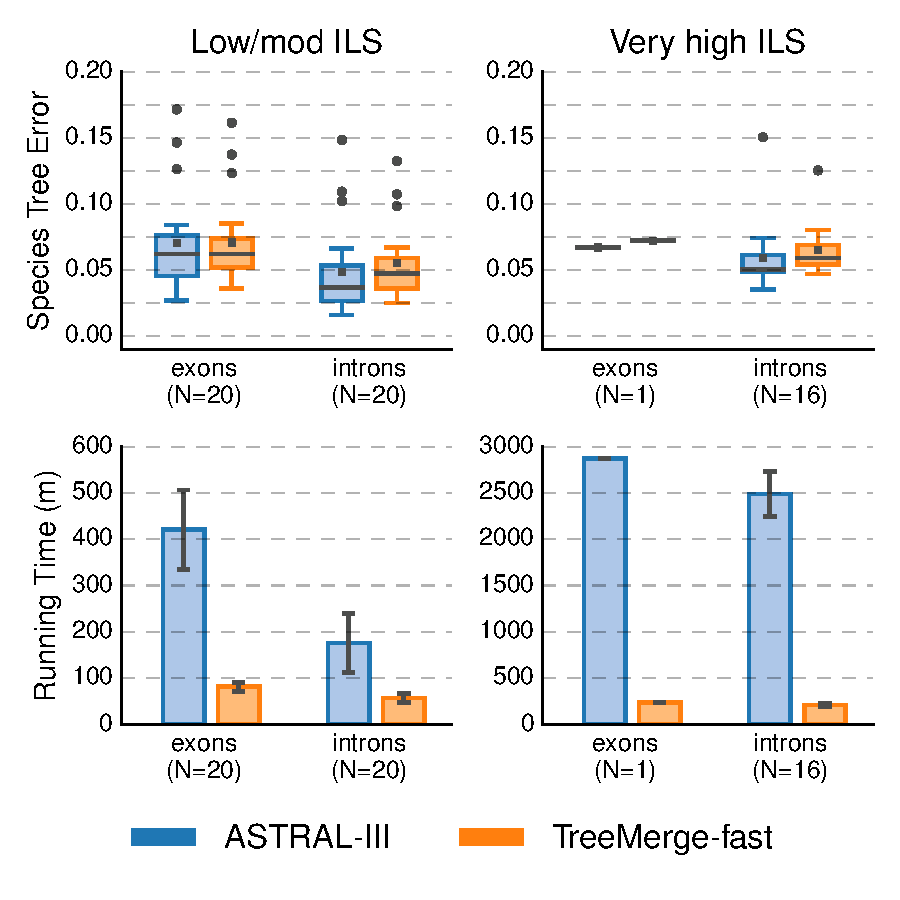
\includegraphics[width=0.8\textwidth]{figures/treemerge-fig4.pdf}
\caption{{\bf Impact of using TreeMerge-fast with ASTRAL-III. }
The top row shows species tree estimation error for datasets with  $1\,000$ species and  $1\,000$ genes. 
Gray bars represent medians, gray squares represent means, gray circles represent outliers, box plots extend from the first to the third quartiles, and whiskers extend to plus/minus 1.5 times the interquartile distance (unless greater/less than the maximum/minimum value).
The bottom row shows running time (in minutes); bars represent means, and error bars represent standard deviations across replicate datasets.
The running time of TreeMerge-fast is the time to estimate the distance matrix, to estimate each subset tree using ASTRAL-III, and to combine the subset trees using TreeMerge-fast (Equation \ref{eq:rt-treemerge}).
The number $N$ of replicates on which ASTRAL-III completed is shown on the $x$-axis; note that averages are taken across the replicates on which ASTRAL-III completed.
When ASTRAL-III did not complete, it was due to running longer than the 48-hour maximum wall-clock time.}
\label{fig:astral}
\end{figure}

%\clearpage

\begin{figure}[!h]
\centering
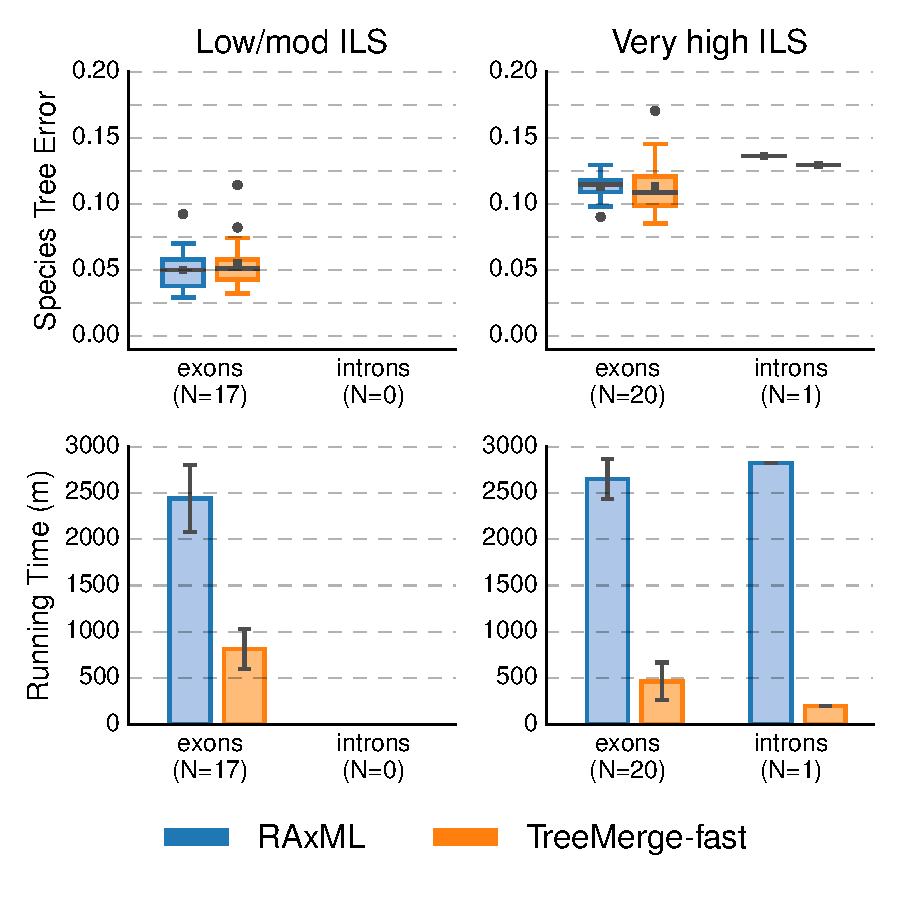
\includegraphics[width=0.8\textwidth]{figures/treemerge-fig5.pdf}
\caption{
{\bf Impact of using TreeMerge-fast with RAxML. }
The top row shows species tree estimation error for datasets with  $1\,000$ species and  $1\,000$ genes. 
Gray bars represent medians, gray squares represent means, gray circles represent outliers, box plots extend from the first to the third quartiles, and whiskers extend to plus/minus 1.5 times the interquartile distance (unless greater/less than the maximum/minimum value).
The bottom row shows running time (in minutes); bars represent means, and error bars represent standard deviations across replicate datasets.
The running time of TreeMerge-fast is the time to estimate the distance matrix, to estimate each subset tree using RAxML, and to combine the subset trees using TreeMerge-fast (Equation \ref{eq:rt-treemerge}).
The number $N$ of replicates on which RAxML completed is shown on the $x$-axis; note that averages are taken across the replicates on which RAxML completed.
When RAxML did not complete, it was due to Out Of Memory (OOM) errors; otherwise the last checkpoint written by RAxML was evaluated.
}
\label{fig:raxml}
\end{figure}

\clearpage

\section{Tables}
\label{sec:treemerge-tables}
This section contains the two tables presented in Section~\ref{sec:treemerge-results} Results.

\vspace{12pt}

\begin{table}[!h]
\caption{{\bf Species tree error for NJMerge vs. NJMerge-2 vs. TreeMerge-fast.}
A comparison of TreeMerge-fast to NJMerge and NJMerge-2 is shown below.
Species tree estimation error (average $\pm$ standard deviation; maximum error is one) is shown for datasets with  $1\,000$ species and  $1\,000$ genes.
The number of replicates on which NJMerge returned a tree is also shown, and averages are taken across the replicates on which NJMerge completed.
When NJMerge failed to return a tree, it was due to algorithmic failure (i.e., considering a siblinghood proposal to be safe when it wasn't).
}
\label{tab:treemerge-s1}
\centering
\begin{tabular}{cccccc}
\toprule
Level of & Data & Number of & NJMerge & NJMerge-2 & TreeMerge-fast \\
ILS & Type & Replicates &  &  & \\
\midrule
\multicolumn{6}{l}{\em ASTRAL-III Analysis (i.e., $M_T$ = ASTRAL-III, $M_D$ = AGID)}\\[0.5ex]
 low/mod & exon & 20 & $0.06 \pm 0.03$ & $0.06 \pm 0.03$ & $0.07 \pm 0.03$\\
 low/mod & intron & 20 & $0.05 \pm 0.03$ & $0.05 \pm 0.03$ & $0.06 \pm 0.03$\\
 very high & exon & 20 & $0.08 \pm 0.04$ & $0.08 \pm 0.04$ & $0.09 \pm 0.03$\\
 very high & intron & 20 & $0.06 \pm 0.02$ & $0.06 \pm 0.02$ & $0.06 \pm 0.02$\\[2ex]
\multicolumn{6}{l}{\em RAxML Analysis (i.e., $M_T$ = RAxML, $M_D$ = log-det)}\\[0.5ex]
 low/mod & exon & 19 & $0.04 \pm 0.02$ & $0.05 \pm 0.02$ & $0.05 \pm 0.02$\\
 low/mod & intron & 20 & $0.03 \pm 0.01$ & $0.03 \pm 0.01$ & $0.04 \pm 0.01$\\
 very high & exon & 17 & $0.10 \pm 0.01$ & $0.10 \pm 0.01$ & $0.11 \pm 0.01$\\
 very high & intron & 18 & $0.09 \pm 0.01$ & $0.09 \pm 0.01$ & $0.10 \pm 0.01$\\
\bottomrule
\end{tabular}
\end{table}

\clearpage

\begin{table}[!h]
\caption{{\bf Running time for each step in divide-and-conquer pipelines using TreeMerge-fast.}
The running time in minutes (mean $\pm$ standard deviation; maximum error is one) is given for each step in the divide-and-conquer pipeline broken down into the time to compute the distance matrix and the time to compute all subset trees and the time to merge the trees together using TreeMerge-fast (i.e., the three terms of Equation~\ref{eq:rt-treemerge}).
We do not show the time required to compute the starting tree, which required just a few minutes for both RAxML and ASTRAL-III analyses.
}
\label{tab:treemerge-s2}
\centering
\begin{tabular}{ccccc}
\toprule
Species Tree & Data & $M_D$ & $M_T$ on all & TreeMerge \\
Height & Type & & subsets &($D$, $\mathcal{T}$) \\
\midrule
\multicolumn{5}{l}{\em ASTRAL-III Analysis (i.e., $M_T$ = ASTRAL-III, $M_D$ = AGID)}\\[0.5ex]
 low/mod & exon & $1 \pm 0$ & $49 \pm 7$ & $32 \pm 5$\\
 low/mod & intron & $1 \pm 0$ & $26 \pm 7$ & $31 \pm 5$\\
 very high & exon & $1 \pm 0$  & $216 \pm 23$ & $33 \pm 6$\\
 very high & intron & $1 \pm 0$ & $178 \pm 19$ & $34 \pm 4$\\[2ex]
\multicolumn{5}{l}{\em RAxML Analysis (i.e., $M_T$ = RAxML, $M_D$ = log-det)}\\[0.5ex]
 low/mod & exon & $24 \pm 1$ & $801 \pm 228$ & $34 \pm 4$\\
 low/mod & intron & $34 \pm 3$ & $1333 \pm 301$ & $32 \pm 4$\\
 very high & exon & $23 \pm 2$ & $412 \pm 199$ & $30 \pm 5$\\
 very high & intron & $40 \pm 3$ & $752 \pm 442$ & $30 \pm 4$\\
\bottomrule
\end{tabular}
\end{table}

\clearpage
